\chapter*{Dodatak: Prikaz aktivnosti grupe}
		\addcontentsline{toc}{chapter}{Dodatak: Prikaz aktivnosti grupe}
		
		\section*{Dnevnik sastajanja}
		
		\textbf{\textit{Kontinuirano osvježavanje}}\\
		
		\begin{packed_enum}
			\item  sastanak
			
			\item[] \begin{packed_item}
				\item Datum: October 19, 2023
				\item Prisustvovali: F.Ljubotina, M.Pavić, A.Vuksanović2, L.Ćorić, K.Klarić, M.Breznički-Herceg, N.Milin
				\item Teme sastanka:
				\begin{packed_item}
					\item  Upoznavanje tima 
					\item  Izrada okvirnog plana rada
				\end{packed_item}
			\end{packed_item}
			
			%
			
		\end{packed_enum}
		
		\eject
		\section*{Tablica aktivnosti}
		
			\textbf{\textit{Kontinuirano osvježavanje}}\\
			
			 \textit{Napomena: Doprinose u aktivnostima treba navesti u satima po članovima grupe po aktivnosti.}

			\begin{longtblr}[
					label=none,
				]{
					vlines,hlines,
					width = \textwidth,
					colspec={X[7, l]X[1, c]X[1, c]X[1, c]X[1, c]X[1, c]X[1, c]X[1, c]}, 
					vline{1} = {1}{text=\clap{}},
					hline{1} = {1}{text=\clap{}},
					rowhead = 1,
				} 
			
				\SetCell[c=1]{c}{} & \SetCell[c=1]{c}{\rotatebox{90}{\textbf{Filip Ljubotina
				}}} & \SetCell[c=1]{c}{\rotatebox{90}{\textbf{Marko Pavić
			 }}} &	\SetCell[c=1]{c}{\rotatebox{90}{\textbf{Ana Vuksanović
		  }}} & \SetCell[c=1]{c}{\rotatebox{90}{\textbf{Lara Ćorić }}} &	\SetCell[c=1]{c}{\rotatebox{90}{\textbf{Katarina Klarić }}} & \SetCell[c=1]{c}{\rotatebox{90}{\textbf{Mihael Breznički-Herceg }}} &	\SetCell[c=1]{c}{\rotatebox{90}{\textbf{Noa Milin
	   }}} \\  
				Upravljanje projektom 		& 8 &  &  &  &  &  & \\ 
				Opis projektnog zadatka 	&  &  &  & 6 &  &  & \\ 
				
				Funkcionalni zahtjevi       &  & 2 &  &  &  &  &  \\ 
				Opis pojedinih obrazaca 	&  & 6 & 2 &  &  &  &  \\ 
				Dijagram obrazaca 			& 5 &  &  &  &  &  &  \\ 
				Sekvencijski dijagrami 		&  &  & 5 &  &  &  &  \\ 
				Opis ostalih zahtjeva 		&  &  &  &  & 1 &  &  \\ 

				Arhitektura i dizajn sustava	 &  & 1.5 &  &  &  &  &  \\ 
				Baza podataka				&  &  &  &  &  & 7 &   \\ 
				Dijagram razreda 			& 2 &  &  &  & 6 &  & 6  \\ 
				Dijagram stanja				&  &  &  &  & 8 &  &  \\ 
				Dijagram aktivnosti 		&  &  &  &  & 7 &  &  \\ 
				Dijagram komponenti			&  &  &  &  &  & 10 &  \\ 
				Korištene tehnologije i alati 		&  & 2 &  &  &  &  &  \\ 
				Ispitivanje programskog rješenja 	& 10 & 10 &  &  &  &  &  \\ 
				Dijagram razmještaja			&  & 1 &  &  &  &  &  \\ 
				Upute za puštanje u pogon 		& 2 &  &  &  &  &  &  \\  
				Dnevnik sastajanja 			& 0.01 &  &  &  &  &  &  \\ 
				Zaključak i budući rad 		&  &  &  & 8 &  &  &  \\  
				Popis literature 			& 0.1 &  &  &  &  &  &  \\  
				&  &  &  &  &  &  &  \\ \hline 
				\textit{izrada back end-a 1. dio } 						& 20 &  &  &  &  &  &  \\  
				\textit{izrada front end-a 1. dio} 			& 5 &  & 15 &  &  &  &  \\ 
				\textit{deploy-anje aplikacije 1. dio} 			& 5 &  &  &  &  &  &  \\
				\textit{izrada back end-a 2. dio } 			& 80 & 40 &  &  &  &  &  \\  
				\textit{izrada front end-a 2. dio} 			& 25 &  & 80 & 40 &  &  &  \\ 
				\textit{deploy-anje aplikacije 2. dio} 			& 2 &  &  &  &  &  &  \\
				\textit{ispravak dijagrama razreda} 			&  &  &  &  &  &  & 8 \\
				\textit{ispravak opisa baze podataka} 			& 3 &  &  &  &  & 8 &  \\
				\textit{ispravak funkcionalnih zahtjeva} 			& 0.5 &  & 3 &  &  & 8 &  \\
				 							&  &  &  &  &  &  &\\ 
			\end{longtblr}
					
					
		\eject
		\section*{Dijagrami pregleda promjena}
		
		\begin{figure}[H]
			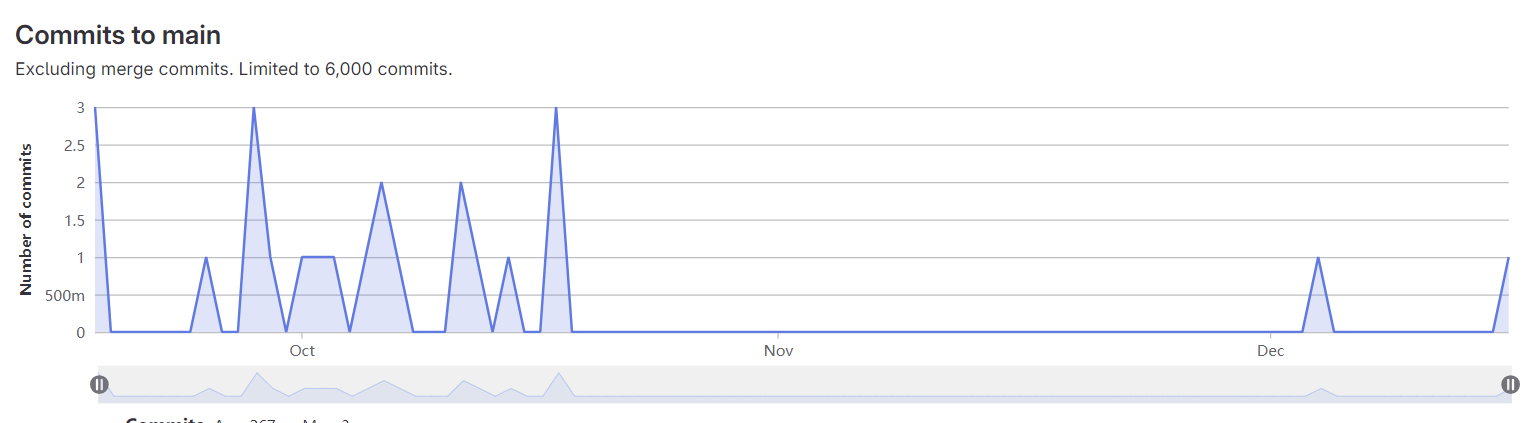
\includegraphics[scale=0.4]{slike/main.png} 
			\centering
			\caption{Promjene na grani main}
			\label{fig:promjene}
		\end{figure}
		
		\begin{figure}[H]
			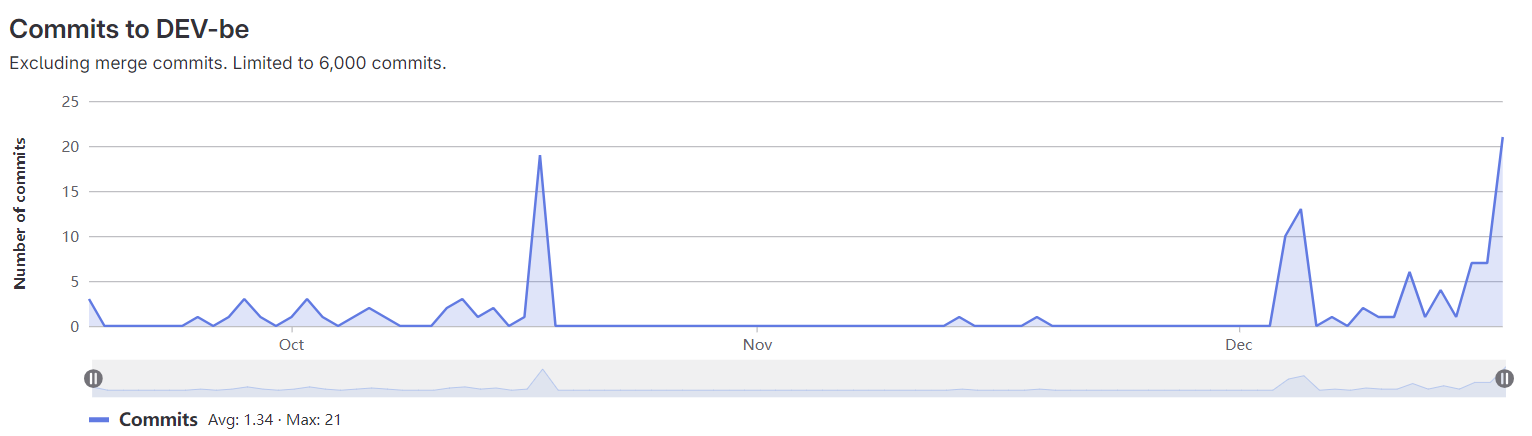
\includegraphics[scale=0.4]{slike/be.png} 
			\centering
			\caption{Promjeve na grani DEV-be}
			\label{fig:promjene}
		\end{figure}
		
		\begin{figure}[H]
			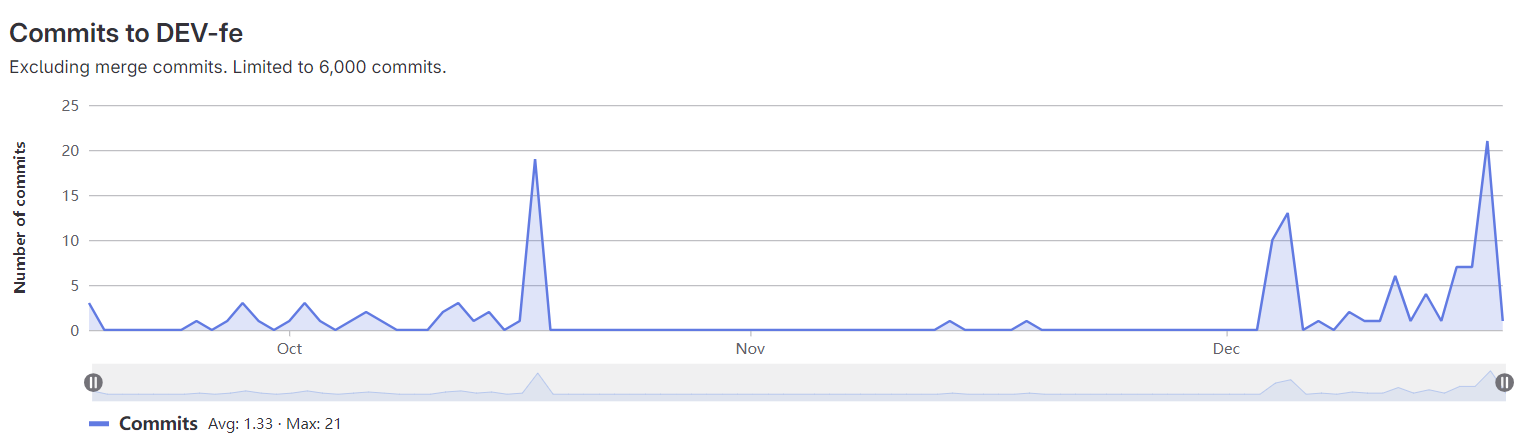
\includegraphics[scale=0.4]{slike/fe.png} 
			\centering
			\caption{Promjeve na grani DEV-fe}
			\label{fig:promjene}
		\end{figure}
		
		\begin{figure}[H]
			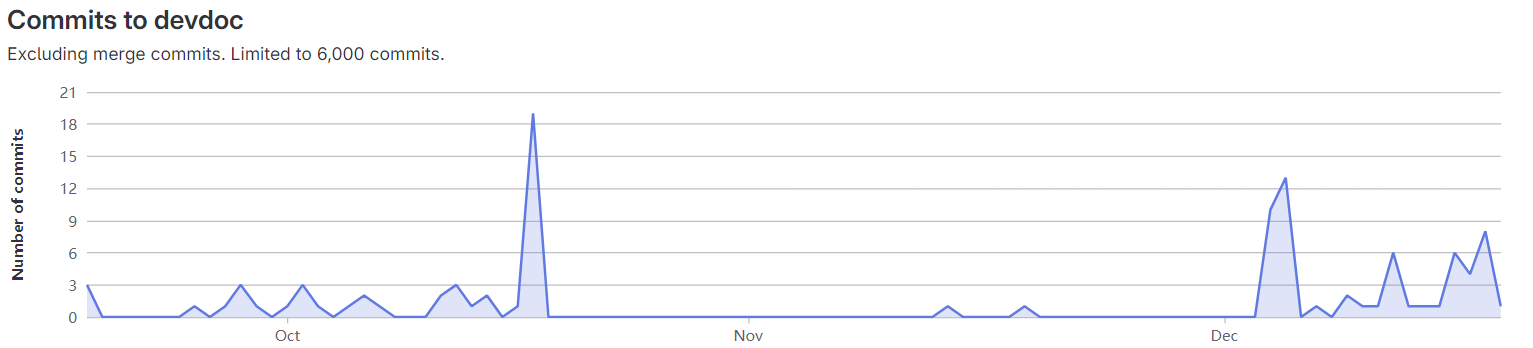
\includegraphics[scale=0.4]{slike/doc.png} 
			\centering
			\caption{Promjeve na grani devdoc}
			\label{fig:promjene}
		\end{figure}
		
	